% This program and the accompanying materials are made available under the
% terms of the MIT license (X11 license) which accompanies this distribution.

% Author: D. Langner, C. Bürger

\chapter{RACR-NET Implementierung: Prozedurale Schnittstelle}\label{umsetzung1}

Dieses Kapitel beschäftigt sich mit der Umsetzung einer prozeduralen Schnittstelle, welche es ermöglicht, RACR in C\# zu nutzen. Zuerst wird gezeigt, wie innerhalb von C\# Scheme-Code aufgerufen und wie die RACR-Scheme-Bibliothek effizient geladen werden kann. Nach einer Anforderungsanalyse wird die Implementierung vorgestellt. Die abschließende Evaluation zeigt die Schwächen einer rein prozeduralen Lösung und leitet zur finalen objektorientierten Lösung im folgenden Kapitel über.

\section{Scheme in C\#}

Mittels der IronScheme-Klassenbibliothek kann Scheme-Code von C\# aus ausgeführt werden. IronScheme bedient sich dazu der Extension-Methoden – ein Feature von C\#, das es erlauben, einem existierenden Typen neue Methoden hinzuzufügen, ohne den ursprünglichen Typ zu manipulieren. Extension-Methoden sind spezielle statische Methoden, die vom Nutzer wie Instanz-Methoden aufgerufen werden.

IronSchemes \csh{Eval} ist eine solche Methode. Sie interpretiert .NET-Strings als Scheme-Ausdrücke und gibt einen Wert vom Typ \csh{object} zurück, dem Basistypen aller .NET-Datentypen. Da C\# statisch typisiert ist, müssen Rückgabewerte zur sinnvollen Weiterverwendung üblicherweise explizit in einen Subtypen konvertiert werden. Deshalb bietet IronScheme auch eine generische Variante der \csh{Eval}-Methode. Diese akzeptiert einen Typ-Parameter, der den Typ des Rückgabewerts festlegt. Die Typumwandlung erfolgt hierbei innerhalb von \csh{Eval}.

Bei Referenztypkonvertierungen wie dieser kann während der Code-Übersetzung nicht bestimmt werden, ob die Umwandlung gültig ist. Schlägt zur Laufzeit eine Typumwandlungsoperation fehl, wird eine \csh{InvalidCastException} ausgelöst. Quelltext~\ref{csh:eval} veranschaulicht die Arbeitsweise von \csh{Eval}.

\begin{lstlisting}[language=csh, caption={Auswerten von Scheme-Ausdrücken}, label=csh:eval]
object a = "(+ 1 2)".Eval();
int b = (int) a;					// explizite Umwandlung
bool c = "(< 3 4)".Eval<bool>();	// generische Methode

bool d = (bool) "(* 2 3)".Eval();	// Laufzeitfehler!
bool e = "(* 2 3)".Eval<bool>();	// Laufzeitfehler!
\end{lstlisting}

Alle Scheme-Prozeduren implementieren das \csh{Callable}"=Interface, mittels welchem man eine Prozedur ohne mehrfaches Parsen oder Kompilieren wiederholt aufrufen kann. Diese abstrakte Klasse stellt \csh{Call}"=Methoden in verschiedenen Ausführungen bereit – variierend über die Anzahl von Parametern, welche wie auch der Rückgabewert stets vom Typ \csh{object} sind. Auf diese Weise wird die dynamische Typisierung von Scheme in C\# abgebildet. Beim Aufruf eines \csh{Callable}"=Objektes kann der Compiler für die korrekte Stelligkeit sowie die Typisierung der Parameter einer Prozedur nicht garantieren. Typfehler äußern sich erst während der Laufzeit eines Programms. Quelltext~\ref{csh:call} zeigt das Interface in Aktion.

\begin{lstlisting}[language=csh, caption={Verwendung des \csh{Callable}"=Interfaces}, label=csh:call]
Callable sum = "+".Eval<Callable>();
int a = (int) sum.Call(1, 2);
int b = (int) sum.Call(3, 4, 5);
int c = (int) sum.Call(0, false);	// Laufzeitfehler!
\end{lstlisting}

\section{RACR in C\#}

\subsection{Importieren der Scheme-Bibliothek}

Der nächste Schritt besteht darin, RACR dem Scheme-Environment bekannt zu machen. RACR laden wir mittels \csh{"(import (racr core))".Eval()}. Dieser Aufruf veranlasst IronScheme dazu, den Quellcode RACRs, der in der Datei \verb|racr/core.sls| residiert, zu kompilieren und alle darin als Export deklarierten Symbole zu registrieren. Dies geschieht mit jedem Neustart des C\#-Programms, was dessen Anlaufzeit verlängert.

Ein weniger dokumentiertes Feature IronSchemes erlaubt es, Scheme-Bibliotheken vorzukompilieren und in Assemblies zu speichern. Auf diese Weise kann das Laden von RACR stark beschleunigt werden. Zum Beispiel lege man eine Datei namens \verb|tmp.scm| mit dem Inhalt \scm{(import (racr core))} an. Der Aufruf von \scm{(compile "tmp.scm")} in der interaktiven IronScheme"=Konsole generiert die Datei \verb|racr.core.dll|. Wenn diese Assembly bei der Kompilierung eines C\#"=Programms referenziert wird, so kompiliert IronScheme RACR mit dem Aufruf von \scm{import} nicht neu, sondern lädt den kompilierten Code aus der DLL"=Datei.

\subsection{Konformitätsprüfung von IronScheme}

Wie im vorhergehenden Kapitel beschrieben, unterscheiden sich Scheme-Interpreter bezüglich ihrer R6RS-Konformität. Um die korrekte Funktion von RACR unter Verwendung verschiedener Interpreter zu gewährleisten, beinhaltet RACR eine Test-Umgebung, die dessen wesentlichen Funktionsumfang abdeckt. Diese Tests wurden mit IronScheme ausgeführt. Dabei terminierten vorerst alle Tests mit dem gleichen Fehler: Der Aufruf von \scm{hashtable-set!} mit dem Schlüssel \scm{'()} löst eine \csh{System.ArgumentNullException} aus. Der Fehler wird durch eine R6RS-Unkonformität IronSchemes verursacht: RACR benutzt häufig die leere Liste als Schlüssel, um Daten in einer \scm{hashtable}"=Datenstruktur abzulegen. Wie Tabelle~\ref{tab:typemapping} zu entnehmen, bildet IronScheme \scm{hashtable} auf den CLI-internen Typ \csh{System.Collections.Hashtable} ab. Des Weiteren wird die leere Liste \scm{'()} auf \csh{null} abgebildet. Laut MSDN\footnote{ \url{https://msdn.microsoft.com/library/system.collections.hashtable.aspx}} darf der Schlüssel eines \csh{Hashtable}"=Objektes jedoch nicht \csh{null} sein.

Ein Workaround in Form einer Scheme-Bibliothek soll bijektiv die leere Liste auf einen internen Record abbilden. Quelltext~\ref{scm:hash} zeigt die Definition dieses Records und dessen Verwendung in den Prozeduren \scm{hashtable-ref*} und \scm{hashtable-set!*}, welche das Interface von \scm{hashtable-ref} beziehungsweise \scm{hashtable-set!} reimplementieren.

\begin{lstlisting}[language=scm, caption={\scm{hashtable}"=Workaround}, label=scm:hash]
(define-record-type nil-record (sealed #t) (opaque #t))
(define nil (make-nil-record))

(define hashtable-ref*
  (lambda (h key default-value)
    (hashtable-ref h (if (null? key) nil key) default-value)))

(define hashtable-set!*
  (lambda (h key value)
    (hashtable-set! h (if (null? key) nil key) value)))
\end{lstlisting}

Auf Zeile~1 wird ein neuer Record-Typ angelegt und anschließend auf Zeile~2 instanziiert. In den Definitionen der \scm{hashtable}"=Prozeduren wird mittels einer \scm{if}"=Anweisung geprüft, ob es sich bei dem Schlüssel um das \scm{null}"=Objekt handelt, in welchem Falle der \scm{nil}"=Record als Schlüssel benutzt werden soll (Zeilen~6 und 10). Auf ähnliche Weise wurde das Interface folgender weiterer Scheme-Prozeduren reimplementiert: \scm{hashtable-delete!}, \scm{hashtable-contains?} und \scm{hashtable-entries}. Diese Bibliothek wurde in RACR eingebunden und alle Aufrufe der genannten Prozeduren auf die entsprechenden Reimplementierungen umgelenkt. Alle Tests der RACR"=Test-Umgebung liefen nun fehlerlos. Somit ist sichergestellt, dass RACR unter IronScheme korrekt ausgeführt wird.

\section{Anforderungsanalyse}\label{anforderungen1}

Um die Qualität der RACR"=C\#"=Schnittstelle bewerten zu können, müssen geeignete Kriterien festgelegt werden. Bislang steht dem Programmierer RACR nur als Scheme-Bibliothek zur Verfügung. Folglich müssen sämtliche Aspekte einer Anwendung, die den Funktionsumfang von RACR nutzen sollen, in Scheme programmiert sein. Mit der Möglichkeit, RACR auch in C\# nutzen zu können, ergeben sich neue Anwendungsfälle, in denen die verschiedenen Aspekte einer RACR-Anwendung zu variierenden Anteilen in Scheme oder C\# implementiert sein können. In einem Beispiel-Szenario werden AST"=Regeln und Attribute einer Sprachspezifikation in Scheme definiert. Mittels dieser Spezifikation werden von C\# aus ASTs instanziiert und Analysen betrieben. Ein weiterer denkbarer Fall ist, dass eine in Scheme spezifizierte Sprache in C\# um zusätzliche Attribute erweitert wird. Abbildung~\ref{fig:usecase} visualisiert diese und weitere Szenarien. Es ergibt sich eine Vielzahl möglicher Varianten der Sprachnutzung, Kopplung und Vererbung und der Aufteilung deren Implementierungen in Scheme und C\#.

Diese Arbeit fokussiert sich auf das Szenario, in dem der Nutzer RACR ausschließlich von C\# aus bedient. Angesichts dessen werden folgende Anforderungen an das System gestellt:

\begin{figure}
	\centering
	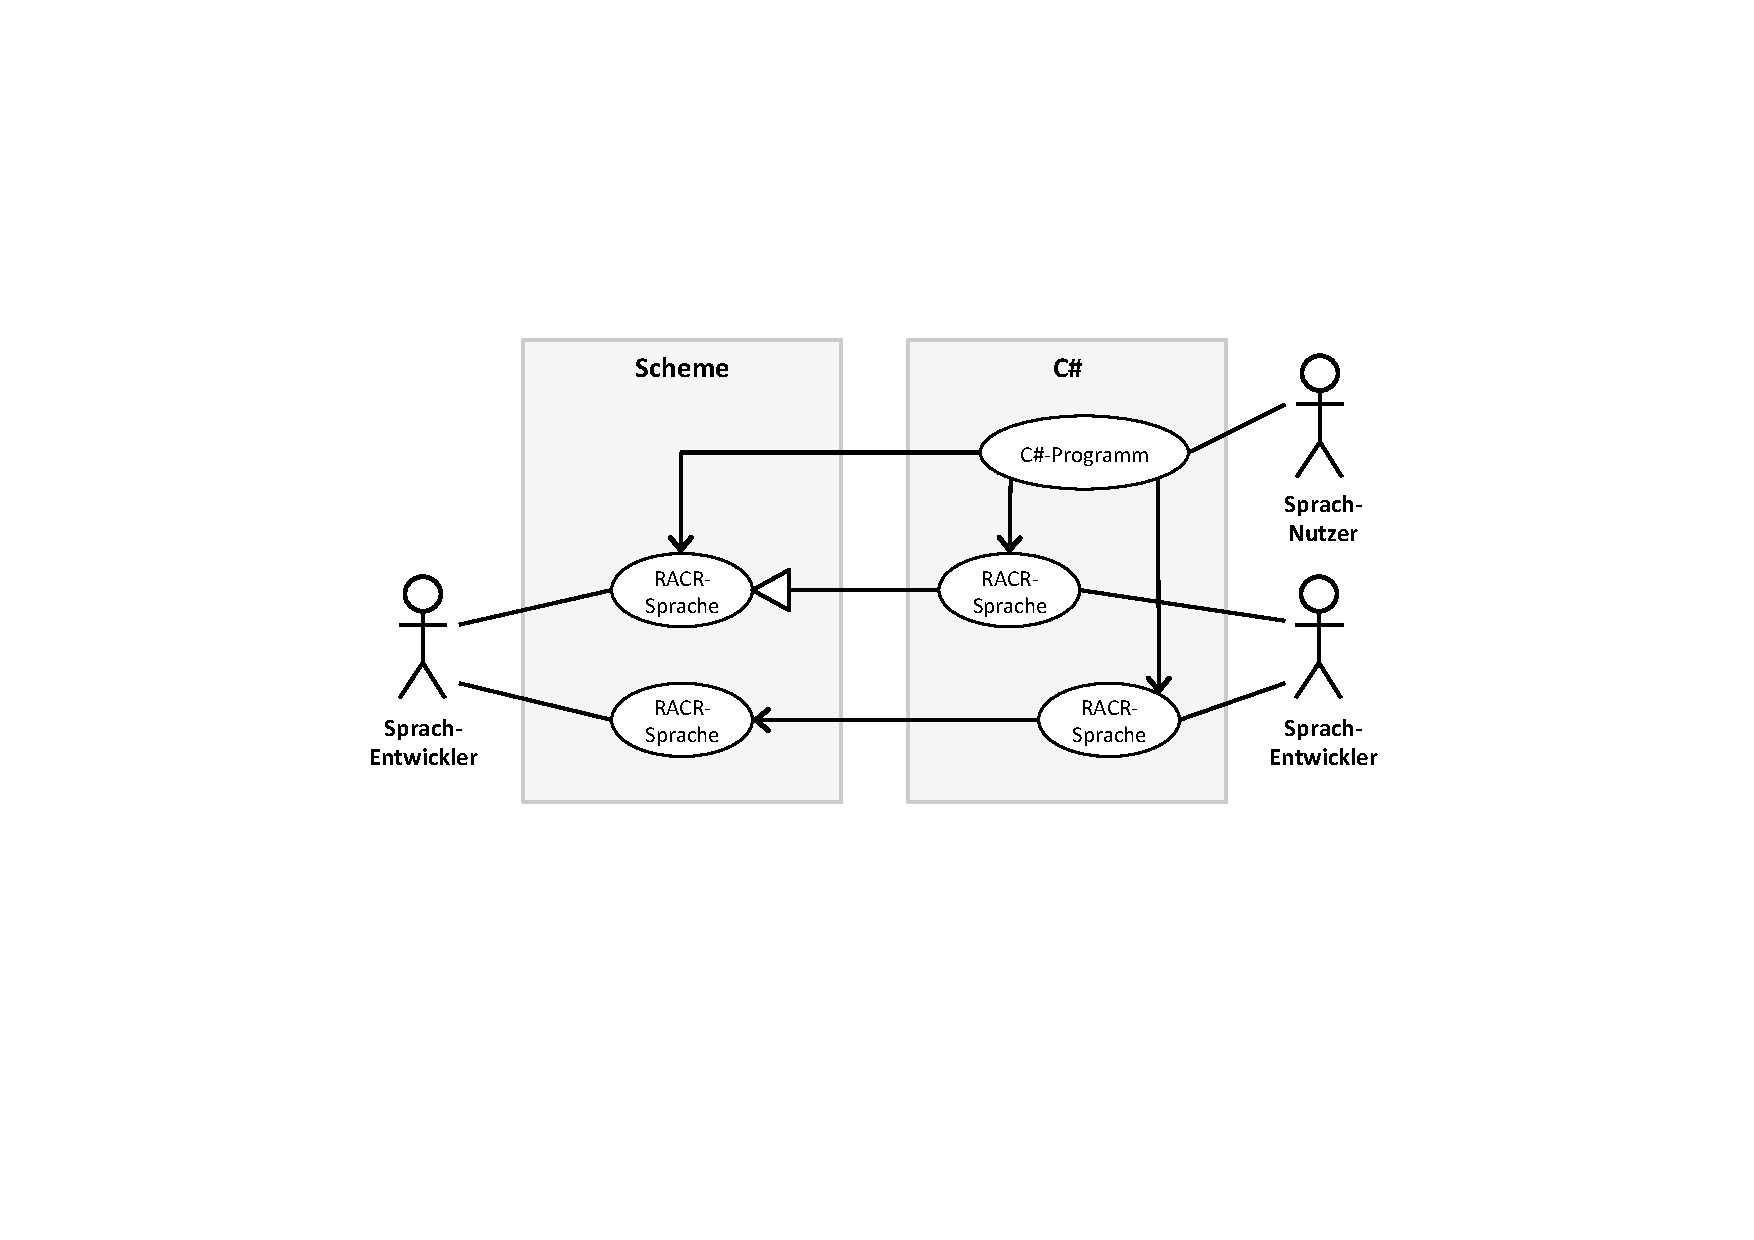
\includegraphics[width=0.9\linewidth]{figures/racr-net-use-cases.pdf}
	\caption{Anwendungsfälle von RACR in Scheme und C\#}
	\label{fig:usecase}
\end{figure}

\begin{description}
	\item[A1 – Vollständigkeit:] Alle dokumentierten~\cite{Buerger2012} Funktionalitäten, die RACR in Scheme bietet, sollen uneingeschränkt auch von C\# aus nutzbar sein.
	\item[A2 – Dynamik:] Die dynamische Natur RACRs muss erhalten bleiben. Grammatik und Attribute sollen noch während der Programmlaufzeit festgelegt werden können. Dies schließt Code-Generatoren, die anhand einer Spezifikation C\#-Code erzeugen, aus.
	\item[A3 – Nähe zur originalen Schnittstelle:] Der Wechsel zwischen Scheme und C\# soll für mit RACR vertraute Programmierer intuitiv sein.
	\item[A4 – Entkoppelung von Scheme:] Dass im Hintergrund die eigentliche Arbeit in einer Scheme-VM passiert, soll für C\#"=Nutzer irrelevant sein und sich in keinster Weise in der Schnittstelle widerspiegeln. Insbesondere sollen IronScheme"=eigene Datentypen, wie zum Beispiel Paare, nicht in der Schnittstelle vorkommen. Stattdessen sollen äquivalente, .NET-typische Typen zum Einsatz kommen.
\end{description}

Im Nachfolgenden soll eine funktionierende, zunächst prozedurale Schnittstelle geschaffen werden, welche die Anforderungen \textbf{A1} bis \textbf{A4} erfüllt. Die endgültige objektorientierte Schnittstelle wird in Kapitel~\ref{umsetzung2} behandelt.

\section{Implementierung der prozeduralen Schnittstelle}

Die prozedurale Schnittstelle soll vollständig sein und die Funktionsweise RACRs nicht einschränken. Ein naiver Ansatz zur Implementierung einer solchen Schnittstelle besteht darin, für jede Scheme-Prozedur in C\# ein direktes Gegenstück zu modellieren – in Form einer statischen Methode. Innerhalb dieser Methoden soll unter Verwendung der IronScheme-VM die entsprechende Prozedur aufgerufen werden. Auf diese Weise werden die Anforderungen \textbf{A1} und \textbf{A2} erfüllt.

Um Anforderung \textbf{A3} zu befriedigen, müssen die Methodennamen denen der zugehörigen Prozeduren gleichen. RACR hält sich bei der Benennung von Variablen beziehungsweise Prozeduren an die für Lisp-Sprachen typischen Konventionen und verwendet in Bezeichnern einige Sonderzeichen. Beispielsweise werden innerhalb eines Bezeichners Worte durch Bindestriche getrennt. Bezeichner von Prozeduren, die einen booleschen Wert liefern, enden für gewöhnlich mit einem Fragezeichen. C\# hat seine eigenen Namenskonventionen. Sonderzeichen in Bezeichnern sind nicht gestattet. Alle Namen öffentlicher Member, Typen und Namespaces beginnen mit einem Großbuchstaben, Parameternamen jedoch mit einem Kleinbuchstaben. Beiderseits werden innerhalb eines Bezeichners verkettete Wörter durch Binnenmajuskel hervorgehoben.

Bei der Benennung der Methoden der .NET-Schnittstelle für RACR soll die C\#-übliche Namenskonvention eingehalten werden ohne den Prozedurnamen zu entfremden. Aus \scm{create-ast} wird \csh{CreateAst}. Alle anderen Benennungen geschehen analog. Somit wird die Realisierung von Anforderung \textbf{A3} gewährleistet. Quelltext~\ref{csh:naiv} skizziert diesen Ansatz.

\begin{lstlisting}[language=csh, caption={Prozedurale C\#"=Schnittstelle für RACR}, label=csh:naiv]
public static class Racr {
	private static Callable createSpecification;
	private static Callable astRule;
	// ...
	static Racr() {
		"(import (racr core))".Eval();
		createSpecification	= "create-specification".Eval<Callable>();
		astRule				= "ast-rule".Eval<Callable>();
		// ...
	}
	public static object CreateSpecification() {
		return createSpecification.Call();
	}
	public static void AstRule(object spec, string rule) {
		astRule.Call(spec, SymbolTable.StringToObject(rule));
	}
// ...
\end{lstlisting}

Die statische Klasse \csh{Racr} umfasst private \csh{Callable}"=Felder, die Referenzen auf die entsprechenden Scheme-Prozeduren RACRs speichern sollen. Im statischen Konstruktor wird zuerst die RACR"=Bibliothek geladen (Zeile~6), woraufhin alle \csh{Callable}"=Objekte initialisiert werden. Zusätzlich enthält die Klasse für jedes \csh{Callable} eine statisch Methode, die als Adapter fungiert, indem sie ihre Argumente an die \csh{Call}"=Methode des entsprechenden \csh{Callable}"=Objekt durchreicht und dessen Rückgabewert zurückliefert. Ein triviales Beispiel hierfür ist die parameterlose Methode \csh{CreateSpecification} (Zeile~11).

\subsection{Entkopplung von Scheme}

Um die Anforderung \textbf{A4} zu erfüllen, werden gegebenenfalls Umwandlungen Scheme-eigener Datentypen erforderlich. RACR nutzt Symbole, Paare und Listen – sowohl für Funktionsparameter als auch für Rückgabewerte. Des Weiteren erwarten einige Prozeduren als Argument selbst eine Prozedur. Der Umgang mit diesen Scheme-typischen Datentypen von C\# aus ist unbequem und ineffizient, weswegen sie in RACRs C\#"=Schnittstelle vermieden werden sollen, sodass der Nutzer nicht mit ihnen konfrontiert wird. An ihrer statt sollen charakteristischere Typen zum Einsatz kommen. Die Implementierung der Schnittstelle muss für die Übersetzung solcher Typen Sorge tragen. Im Folgenden soll auf jene Datentypen eingegangen werden, die zur Verarbeitung in C\# einer Sonderbehandlung bedürfen.

\subsubsection{Symbole}

Scheme-Symbole tauchen in RACRs Schnittstelle an vielen Stellen auf. Aufseiten von C\# sollen stattdessen .NET-Strings zum Einsatz kommen. Symbole werden unter anderem als Zeichenketten für Nichtterminale, ganze AST-Regeln und Attributsnamen verwendet. IronScheme implementiert Symbole mittels der Struktur \csh{SymbolId}, deren \csh{ToString} Methode die String-Repräsentation der jeweiligen Symbol-Instanz liefert. Analog bildet die statische Methode \csh{SymbolTable.StringToObject} Strings auf Symbole ab. Quelltext~\ref{csh:naiv} zeigt die Verwendung von \csh{SymbolTable.StringToObject} in der Methode \csh{AstRule} (Zeile~15).

\subsubsection{Paare}

Paare sind in Scheme ein essenzieller Datentyp. In RACRs Scheme"=Schnittstelle kommen Paare in folgenden Prozeduren zum Einsatz: \scm{ast-children}, \scm{ast-for-each-child}, \scm{ast-find-child} und \scm{ast-find-child*}. Diese Prozeduren verlangen neben anderen Arguenten eine unbestimmte Anzahl von sogenannten Kinder-Intervallen – Paare, die in Form von zwei Indices eine untere und ober Grenze enthalten. Mit dem Scheme-Symbol \scm{'*} kann auch eine offene obere Grenze angegeben werden\footnote{\url{https://github.com/christoff-buerger/racr/blob/master/documentation/abstract-syntax-trees.md\#ast-children}}. Paare entsprechen in C\# Objekten der Klasse \csh{Cons} aus der IronScheme-Klassenbibliothek. Nutzer sollen mit ihr nicht in Berührung kommen müssen, sondern zur Angaben von Kinder-Intervallen eine für genau diesen Zweck geschaffene Datenstruktur verwenden. Quelltext~\ref{csh:range} zeigt die dafür konzipierte Struktur \csh{Range}.

\begin{lstlisting}[language=csh, caption={Definition der \csh{Range}"=Struktur}, label=csh:range]
public struct Range {
	public int min;
	public int max;
	public Range(int min, int max=0) {
		this.min = min;
		this.max = max;
	}
	internal Cons ToCons() {
		return new Cons(min,
						max > 0 ? max : SymbolTable.StringToObject("*"));
	}
}
\end{lstlisting}

Zweckmäßig hält die Struktur zwei Felder für die beiden Grenzen, wobei eine obere Grenze mit dem Wert 0 als offen interpretiert wird\footnote{In RACR werden Indices stets von 1 an gezählt.}. Die interne Methode \csh{ToCons} dient dazu, aus dem \csh{Range}"= ein \csh{Cons}"=Objekt zu konstruieren, das von IronScheme aus weiterverarbeitet werden kann. Sie kommt in den Methoden des Interfaces, welche die oben genannten Prozeduren abbilden sollen, zum Einsatz.

\subsubsection{Listen}

Scheme-Listen sind verschachtelte Scheme-Paare. Sie sind ein Parameter der Prozeduren \scm{create-ast} und \scm{create-ast-list} und der Rückgabetyp der Prozeduren \scm{ast-children} und \scm{rewrite-abstract}. Analog zu \scm{create-ast-list}, erwartet die \scm{create-ast} als letztes Argument eine Liste mit den Kindern des zu erzeugenden AST-Knoten. In der C\#"=Schnittstelle soll für den Nutzer der Zwischenschritt, erst eine Liste für die Kinder zu konstruieren, übersprungen werden. Stattdessen soll die Methode \csh{CreateAst} ein C\#"=Array von Kind-Knoten akzeptieren. Unter Verwendung einer einfachen Schleife über das Array soll daraus die Scheme-Liste erzeugt werden, damit sie anschließend beim Aufruf der Scheme-Prozedur übergeben werden kann.

\begin{lstlisting}[language=csh, caption={Listenkonstruktion in \csh{CreateAst}}, label=csh:createast]
public static object CreateAst(object spec, string nonTerm,
							   params object[] children)
{
	Cons list = null;
	for (int i = children.Length - 1; i >= 0 ; i--) {
		list = new Cons(children[i], list);
	}
	return createAst.Call(spec, SymbolTable.StringToObject(nonTerm),
						  list);
}

\end{lstlisting}

Quelltext~\ref{csh:createast} zeigt die Implementierung der Methode \csh{CreateAst} der Klasse \csh{Racr} gemäß den oben genannten Vorgaben. Man beachte, dass dem Parameter \csh{children} das Schlüsselwort \csh{params} vorangestellt ist. Es bewirkt, dass beim Aufruf der Methode eine variable Anzahl von Methodenargumenten automatisch zu einem Array zusammengefasst wird, sodass der Nutzer das Array nicht selbst anzulegen braucht. Will man beispielsweise einen Knoten mit drei Kind-Knoten erzeugen, gestaltet sich der Aufruf von \csh{CreateAst} wie folgt:

\begin{lstlisting}[language=csh, numbers=none]
object node = Racr.CreateAst(spec, "A", childA, childB, childC);
\end{lstlisting}

Auch als Rückgabewert sollen in der C\#"=Schnittstelle Scheme-Listen durch Arrays ersetzt werden. Die in Quelltext~\ref{csh:rewriteabstract} abgebildete Implementierung von \scm{RewriteAbstract} nutzt eine \csh{while}"=Schleife, um die Kette von \csh{Cons}"=Objekten zu durchwandern und die in der Liste gespeicherten Kind-Knoten einer \csh{List<object>} anzuhängen. Die Klasse \csh{List} ist Teil der .NET-Klassenbibliothek. Im Gegensatz zum Array bietet sie Methoden, um die Anzahl ihrer Elemente dynamisch zu ändern.

\begin{lstlisting}[language=csh, caption={Arraykonstruktion in \csh{RewriteAbstract}}, label=csh:rewriteabstract]
public object[] RewriteAbstract(string supertype) {
	var list = rewriteAbstract.Call(ast,
			   SymbolTable.StringToObject(supertype)) as Cons;
	var children = new List<object>();
	while (list != null) {
		children.Add(list.car);
		list = list.cdr as Cons;
	}
	return children.ToArray();
}
\end{lstlisting}

\subsubsection{Prozeduren}\label{prozeduren}

Schemes Prozeduren sind First-Class-Objekte und können Funktionen als Argumente überreicht werden. Insofern ist Scheme eine höhere, funktionale Sprache. Wie schon erwähnt, sind Prozeduren aus der Sicht von .NET Subtypen der abstrakten Klasse \csh{Callable}. C\# unterstützt First-Class-Funktionen in Form von Delegaten – Referenztypen, mit denen eine benannte oder anonyme Methode gekapselt werden kann. Sie haben Ähnlichkeit mit Funktionszeigern in C. Der Typ eines Delegat-Objektes entspricht einer bestimmten Methodensignatur, die sich aus der Anzahl und den Typen der Parameter und dem Rückgabetyp zusammensetzt. Um C\#"=Methoden an RACR zu übergeben, müssen diese zuerst in ein \csh{Callable} umgewandelt werden. IronScheme bietet zu diesem Zweck die Extension-Methode \csh{ToSchemeProcedure} der Klasse \csh{Delegate}, die Basisklasse aller Delegat-Typen. Innerhalb von RACR erwarten folgende Prozeduren eine Funktion als Argument: \scm{ast-for-each-child}, \scm{ast-find-child}, \scm{ast-find-child*} und \scm{specify-attribute}. Dabei gleichen sich die ersten drei insofern, dass die Signatur der zu übergebenden Prozedur von RACR vorgegeben ist, woraus sich für die C\#"=Schnittstelle ein entsprechender Delegat-Typ ergibt.

\begin{lstlisting}[language=csh, caption={Delegat-Parameter in \csh{AstFindChild}}, label=csh:astfindchild]
public static object AstFindChild(object node, Func<int,object,bool> f,
								  params Range[] bs)
{
	object[] args = new object[2 + bs.Length];
	args[0] = f.ToSchemeProcedure();
	args[1] = node;
	for (int i = 0; i < bs.Length; i++) args[i + 2] = bs[i].ToCons();
	object res = astFindChild.Call(args);
	if (res is bool && (bool) res == false) return null;
	return res;
}
\end{lstlisting}

Quelltext~\ref{csh:astfindchild} zeigt die Implementierung von \csh{AstFindChild}. Die Methode ist variadisch, genau wie die Scheme-Prozedur, an die sie ihre Argumente weiterleiten muss. Um eine unbestimmte Anzahl von Argumenten an den Aufruf eines \csh{Callable}"=Objekts weiterzugeben, müssen diese in ein Objekt-Array geschrieben werden, welches als einziger Parameter an \csh{Call} übergeben werden muss. Zeile~4 deklariert dieses Array und die drei darauffolgenden Zeilen befüllen es. Dem Delegat-Typen \csh{Func<int,object,bool>} zufolge muss die zu übergebende Funktion zwei Parameter mit den Typen \csh{int} und \csh{object} für den Index des Knoten beziehungsweise den Knoten selbst habe, nebst dem Rückgabetypen \csh{bool}. \csh{ToSchemeProcedure} nutzt die durch Introspektion zugänglichen Typinformationen, um ein \csh{Callable}"=Objekt zu generieren, in welchem der Delegat gekapselt wird. Die Methode \csh{AstFindChild} weicht in ihrem Verhalten von \scm{ast-find-child} ab, indem sie bei einer missglückten Suche statt \csh{false} \csh{null} zurückgibt (Zeile~9). Dies entspricht der in C\# üblichen Weise, das Fehlen eines Objektes zu kennzeichnen.

Der Aufruf von \csh{AstFindChild} gestaltet sich unter Benutzung von C\#'s Lambda-Ausdrücken elegant. Hier ein Beispiel:

\begin{lstlisting}[language=csh]
object child = Racr.AstFindChild(parent, (i, n) => {
		bool success;
		// setze success anhand von Attributsauswertungen, etc.
		return success;
	}, new Racr.Range(2, 7));
\end{lstlisting}

Mit \scm{specify-attribute} lassen sich (gegebenenfalls Referenz-) Attribute definieren. Dieser Prozedur muss dabei unter anderem eine Attributgleichung (in Form eines Delegaten) übergeben werden. RACR unterstützt parametrisierte Attribute, was sich darin äußert, dass die Attributgleichungsfunktion neben einem Argument für den AST-Knoten noch weitere Argumente akzeptiert, mit welchem die auszuwertende Instanz des Attributes assoziiert ist. Bei der Attributsauswertung mittels \scm{att-value} muss die entsprechende Anzahl an Argumenten des Attributs mit übergeben werden. Für die Korrektheit der Argumenttypen ist stets der Programmierer allein verantwortlich.

Aus der Sicht einer statisch typisierten Sprache wie C\# stellt diese Dynamik in der Attributsspezifikation und -auswertung eine Herausforderung dar, da der exakte Typ der Attributgleichungsfunktion beinahe beliebig sein kann: Nur der erste Parameter wird von RACR als AST-Knote vorgegeben. Die Implementierung der Methodengruppe \csh{SpecifyAttribute}\footnote{Der Einfachheit halber ist hier eine Implementierung gezeigt, die keine zyklischen Attribute unterstützt.} ist in Quelltext~\ref{csh:specifyattribute} abgebildet. Die erste Methode besitzt für die Attributgleichung einen Parameter vom Typ \csh{Delegate}. Lambda-Ausdrücke werden vom Compiler jedoch nicht implizit nach \csh{Delegate} umgewandelt. Um den Nutzer dennoch von verbosen Typumwandlungen zu entlasten, decken die zwei zusätzlichen generischen Ausführungen von \csh{SpecifyAttribute} den Fall für parameterlose (\csh{Func<object,R>}) beziehungsweise mit einem Parameter parametrisierte (\csh{Func<object,T,R>}) Attribute ab.

\begin{lstlisting}[language=csh, caption={Methodengruppe \csh{SpecifyAttribute}}, label=csh:specifyattribute]
public static void SpecifyAttribute(object spec, string name,
		string nonTerm, string context, bool cached, Delegate eq)
{
	specifyAttribute.Call(spec,
						  SymbolTable.StringToObject(name),
						  SymbolTable.StringToObject(nonTerm),
						  SymbolTable.StringToObject(context),
						  cached,
						  eq.ToSchemeProcedure(),
						  false);
}
public static void SpecifyAttribute<R>(object spec, string name,
		string nonTerm, string context, bool cached, Func<object,R> eq)
{
	SpecifyAttribute(spec, name, nonTerm, context, cached, (Delegate) eq);
}
public static void SpecifyAttribute<T,R>(object spec, string name,
		string nonTerm,	string context, bool cached, Func<object,T,R> eq)
{
	SpecifyAttribute(spec, name, nonTerm, context, cached, (Delegate) eq);
}
\end{lstlisting}

Um den Einsatz von \csh{SpecifyAttribute} vorzuführen, definiert folgender C\#"=Code das parameterlose Attribut \verb|value| für den Knotentypen \verb|Addition|:

\begin{lstlisting}[language=csh]
Racr.SpecifyAttribute(spec, "Eval", "Addition", "*", true, (n) => {
	return (int) Racr.AttValue(Racr.AstChild(n, 1), "value")
		 + (int) Racr.AttValue(Racr.AstChild(n, 2), "value");
});
\end{lstlisting}

Dies entspricht folgender Attributspezifikation in Scheme:

\begin{lstlisting}[language=scm]
(with-specification spec
  (ag-rule
    value
    (Addition
      (lambda (n)
        (+ (att-value 'value (ast-child 1 n))
           (att-value 'value (ast-child 2 n)))))))
\end{lstlisting}

\subsection{Evaluation der Schnittstelle}\label{evaluation1}

Die resultierende Schnittstelle deckt den vollständigen Funktionsumfang RACRs ab (\textbf{A1}). Sprachspezifikationen können zur Programmlaufzeit dynamisch definiert werden (\textbf{A2}). Obschon die Schnittstelle sehr dem Original ähnelt (\textbf{A3}), wird der Nutzer zu keiner Zeit mit konkreten Scheme-Typen konfrontiert (\textbf{A4}).

Die Schnittstelle hat jedoch zwei entscheidende Schwächen: Für Sprachspezifikationen und AST-Knoten fehlen konkrete Typen. Die entsprechenden RACR-spezifischen Objekttypen, auf denen alle RACR-Prozeduren arbeiten, sind Scheme-Records mit den Namen \scm{ast-specification} beziehungsweise \scm{node}. Diese Datentypen werden erst zur Programmlaufzeit generiert. IronScheme kann für Instanzen solcher Typen keinen präziseren Subtypen als \csh{object} geben. Effektiv handelt es sich hierbei um opake Handler, ähnliche den \csh{void}–Zeigern in C. Deshalb sind Spezifikationen sowie AST-Knoten in der Schnittstelle stets als \csh{object} typisiert. Konsequenterweise ist aus der Signatur einer RACR-Methode allein nicht klar ersichtlich, welcher tatsächliche Objekttyp erwartet wird, was eine Quelle von Typfehlern darstellt, die während der Übersetzung nicht erkannt werden können.

Eine weitere Schwachstelle besteht in der Benutzerfreundlichkeit der Schnittstelle, die dem Nutzer einen prozeduralen Programmierstil aufdrängt. Objektorientierung, die Grundcharakteristik von C\#, wird nicht wirkungsvoll eingesetzt.

Aus den vorgestellten Nachteilen ergeben sich die folgenden zusätzlichen Anforderungen an die bereits in Kapitel~\ref{anforderungen1} präsentierten:

\begin{description}
	\item[A5 – Entkoppelung von der RACR-Implementierung:] Der Nutzer soll nicht direkt mit den Handlern für \scm{ast-specification} und \scm{node} arbeiten. Opake RACR-Datentypen sollen in Stellvertreter-Objekten gekapselt werden.	
	\item[A6 – Objektorientierung:] Alle wesentlichen Prozeduren von RACR können entweder Spezifikationen oder AST-Knoten zugeordnet werden. Die C\#"=Schnittstelle soll diese Prozeduren als Methoden der entsprechenden Objekte bereitstellen.
\end{description}
